\documentclass[12pt,a4paper,oneside]{report}
\usepackage[margin=25mm,headheight=15pt]{geometry}
\usepackage{setspace}
\onehalfspacing
\usepackage[T1]{fontenc}
\usepackage[utf8]{inputenc}
\usepackage{lmodern}
\usepackage{microtype}
\usepackage{graphicx}
\graphicspath{{figures/}}
\usepackage{booktabs,tabularx,array,longtable}
\usepackage{amsmath,amssymb}
\usepackage{float}
\usepackage{caption}
\usepackage{subcaption}
\usepackage{xcolor}
\usepackage{fancyhdr}
\usepackage{enumitem}
\usepackage{hyperref}
\usepackage[nameinlink,noabbrev]{cleveref}
\usepackage[numbers,sort&compress]{natbib}
\hypersetup{colorlinks=true,linkcolor=black,citecolor=blue!55!black,urlcolor=blue!55!black,pdftitle={A Comparative Study of RAG Techniques for Generating Image Captions},pdfauthor={University Project}}
\pagestyle{fancy}\fancyhf{}\fancyhead[L]{\nouppercase{\leftmark}}\fancyhead[R]{Phase 1 Report}\fancyfoot[C]{\thepage}\setlength{\parskip}{0.35em}
\setcounter{secnumdepth}{3}\setcounter{tocdepth}{2}
\emergencystretch=2em
\newcommand{\pending}{\textit{Pending experiment}}
\newcommand{\phaseone}{\textsc{Phase 1}}
\begin{document}
\begin{titlepage}\centering\vspace*{22mm}
{\Large Academic Technical Report\par}\vspace{18mm}
{\huge\bfseries A Comparative Study of RAG Techniques for Generating Image Captions\par}\vspace{12mm}
{\Large Dataset Exploration, Preprocessing, and Retrieval Infrastructure\par}\vspace{24mm}
\begin{tabular}{rl}Student: & [Student name]\\Programme: & [Programme / Department]\\Institution: & [University]\\Supervisor: & [Professor / Supervisor]\\Date: & November 2026\end{tabular}
\vfill\begin{minipage}{0.88\textwidth}\small\textbf{Scope statement.} This document reports the repository's completed data preparation and retrieval infrastructure. Caption generation, comparisons among RAG methods, and generated-caption evaluation have not yet been implemented.\end{minipage}\vspace{15mm}\end{titlepage}
\pagenumbering{roman}\tableofcontents\listoffigures\listoftables\clearpage\pagenumbering{arabic}
\chapter*{Abstract}\addcontentsline{toc}{chapter}{Abstract}
This report documents the implemented first phase of a project on retrieval-augmented image captioning. Using MS COCO 2017, the repository freezes 10,000 training images, 100 validation images, and 1,000 test images, each with five human reference captions. A reproducible preprocessing pipeline creates 224 by 224 RGB letterboxed images. Annotation-derived metadata, caption statistics, geometric analyses, image and text representations from CLIP ViT-B/32, and separate training-only FAISS indexes provide a foundation for downstream retrieval-augmented caption generation. Integrity checks report 11,100 decoded images, no split overlap, no exact SHA-256 duplicate groups, no cross-split perceptual-hash candidates at Hamming distance at most six, and valid embedding/index mappings. A smoke evaluation retrieves the top five training images for 20 held-out queries, with no self-matches and mean top-1 cosine similarity 0.8260. This is retrieval validation, not evidence of improved caption quality. No generator, comparative RAG treatments, statistical comparison, ablation, or hallucination-rate experiment exists in the repository. Those sections are therefore explicitly framed as planned work. The supplied project specification reports a conflict between 100 and 1,000 test images; the frozen implementation retains 1,000. The original assignment PDF could not be located, which limits direct verification of its exact wording.
\textbf{Keywords:} image captioning; retrieval-augmented generation; MS COCO; CLIP; FAISS; data integrity.

% Compatibility entry point; active chapter source: chapter1_introduction.tex.
\section{Introduction and Project Objectives}
\label{ch:introduction}

Image captioning is the task of describing an image in a short natural-language sentence. A useful caption names important objects and may describe their attributes, actions, or relationships. A caption should also avoid details that are not supported by the image. Current vision-language systems can produce fluent text, but fluent wording alone does not guarantee that the details are correct.

Retrieval-Augmented Generation (RAG) is a design in which a system retrieves information from a separate collection and uses it when generating an answer \citep{lewis2020rag}. For image captioning, the retrieved material could include visually similar training images, captions written for those images, or structured visual metadata. The retrieved examples may guide a caption generator, but they may also introduce incorrect objects or relationships. Their effect must be measured rather than assumed.

\subsection{Objective}
The project asks how retrieval techniques affect caption quality, relevance, and grounding. This report covers Phase 1: the data, metadata, embedding, and retrieval foundation. It does not generate captions or compare RAG methods.

\endinput
\chapter{Introduction and Problem Statement}\label{ch:intro}
Image captioning maps a visual scene to a concise natural-language description. A useful caption must identify salient entities, their attributes, and relevant relations while avoiding details unsupported by the image. Modern vision-language encoders provide transferable representations, but caption generation remains sensitive to data coverage, retrieval quality, decoder behavior, and evaluation design. Retrieval-augmented generation (RAG) introduces external examples or knowledge at inference time, potentially giving a generator access to information beyond its parametric weights \cite{lewis2020rag}.

The project title proposes a comparative study of RAG techniques for generating image captions. The implemented repository currently supplies important groundwork: fixed data splits, five references per image, visual and linguistic analyses, CLIP representations, and train-only similarity indexes. Its present status must be understood as an infrastructure and data-preparation phase, not the completed comparative study. This distinction governs every result reported here.

The report has three aims. First, it describes the code and artifacts that exist, rather than treating the project title as proof of completed experiments. Second, it summarizes verified properties of the dataset and retrieval pipeline. Third, it specifies how the pending generation study can be conducted without implying that proposed metrics or outcomes have already been measured.

\section{Problem Statement}\label{ch:problem}
The intended research question is whether retrieval-augmented captioning methods can improve the quality and factual grounding of image captions relative to a non-retrieval baseline. Answering it requires (i) selecting comparable caption generators and RAG strategies, (ii) retrieving relevant evidence without test leakage, (iii) generating captions under controlled decoding settings, and (iv) evaluating linguistic quality and visual faithfulness on held-out images. The repository has completed only part of the second requirement: it creates train-only image and caption vector indexes and checks image-neighbor retrieval.

The current operational problem is therefore narrower: can the project assemble a stable, audited COCO subset and produce correctly mapped visual/text representations and retrieval structures suitable for later experiments? The recorded evidence supports a positive answer for the implemented Phase 1 checks. It does not establish a causal effect of retrieval on generated captions.

\section{Research questions and scope}
The completed phase addresses data integrity and pipeline feasibility. It does not answer which RAG method performs best, whether RAG reduces hallucinations, or whether improvements are statistically significant. Those are Phase 2 questions. The available retrieval smoke test reports embedding similarity, not reference-caption agreement or factual correctness.

\section{Test-size requirement}
The original assignment's detailed dataset and preprocessing requirements specify 1,000 test images. One occurrence contains the typographical value \code{1,00}; the detailed requirements and data-audit instructions establish 1,000 as intended. The frozen split contains 1,000 test images and is unchanged.

% Compatibility entry point; active section source: concepts.tex.
\section{Key concepts}
\label{sec:concepts}

\subsection{Image and caption retrieval}
An \emph{embedding} is a list of numbers that represents an image or a text caption. Embeddings from a shared model can be compared to find items with similar representations. In this project, the image encoder is used to retrieve training images similar to a held-out query image. The caption index stores vectors for training captions, but a caption-generation pipeline that uses these results has not been implemented.

\subsection{What similarity does and does not mean}
The project uses CLIP, a vision-language model trained to align image and text representations \citep{radford2021clip,clipmodelcard}. A high similarity score means that two vectors are close under the chosen representation. It does not prove that the retrieved image is an exact match, that its caption applies to the query, or that a future generated caption is factually correct.

FAISS is a library for efficient similarity search over vectors \citep{douze2024faiss,faissdocs}. The project uses its exact flat inner-product index. Because the stored vectors are L2-normalized, inner product gives cosine similarity. This index provides a straightforward reference search, not an approximate search optimization.

\subsection{Phase boundaries}
Phase 1 ends with saved splits, analysis, embeddings, indexes, and retrieval checks. Phase 2 must add a generator, define retrieval conditions and prompts, run controlled generation, and evaluate the outputs. The two phases should not be confused when interpreting the results in this report.

\endinput
\chapter{Background and Assigned Technique}\label{ch:sota}
\section{Retrieval-augmented generation}
RAG combines a retriever over non-parametric memory with a generator that conditions on retrieved material. In the original formulation, dense retrieval selects passages and a sequence-to-sequence model conditions on them for knowledge-intensive NLP tasks \cite{lewis2020rag}. Subsequent work has explored retrieval over examples, documents, demonstrations, and multimodal content. For image captioning, retrieved items may be similar images, their captions, structured annotations, or combinations of these. These choices are not interchangeable: image-neighbor retrieval can provide visual analogies, while caption retrieval can offer lexical templates but may also transfer incorrect objects or relations.

The project implements vector indexes that could support example retrieval, but it does not yet implement a generator that consumes retrieved records. Consequently, the current system is a retrieval-capable dataset pipeline rather than a complete RAG model. A meaningful comparison must specify retrieval query, candidate corpus, top-$k$, filtering, prompt construction, generator, decoding, and controls.

\section{Image captioning and evaluation}
COCO has been widely used to study object recognition and image captioning in complex everyday scenes \cite{lin2014coco}. Its multiple captions per image capture some of the diversity of human descriptions, but references are not exhaustive descriptions of every visible fact. N-gram metrics such as BLEU and ROUGE-L measure overlap with references; METEOR adds stemming and synonym-aware matching; CIDEr emphasizes consensus with multiple references; SPICE compares semantic scene-graph propositions; learned similarity measures such as BERTScore compare contextual token representations \cite{papineni2002bleu,banerjee2005meteor,lin2004rouge,vedantam2015cider,anderson2016spice,zhang2020bertscore}. Each metric captures a different aspect and none alone establishes visual truth. The repository has not generated captions and reports none of these scores.

\section{Vision-language representations}
CLIP learns aligned image and text spaces through contrastive image-text pretraining and supports transfer using natural-language supervision \cite{radford2021clip}. This makes CLIP embeddings a practical common representation for image and caption similarity. Similarity is not equivalent to caption correctness: semantically related images may differ in small objects, counts, actions, or spatial relations. In this project CLIP is used for embedding and zero-shot exploratory predictions; those predictions are not ground-truth annotations.

\section{Assigned Technique and Implemented Method}\label{ch:method}
The assignment's exact designated RAG technique cannot be identified from the source PDF because that file was not found. The supplied task text names a comparative RAG study but does not provide a verifiable technique assignment. Rather than invent an assigned method, this report describes the repository's actual method: dense cosine retrieval using CLIP embeddings and exact inner-product search, with separate image and caption memories. No caption-generation strategy has been selected or implemented.

For an image representation $q$ and training representation $v_i$, retrieval ranks candidates by cosine similarity
\begin{equation}\label{eq:cosine}
 s(q,v_i)=\frac{q^\top v_i}{\lVert q\rVert_2\lVert v_i\rVert_2}.
\end{equation}
Embeddings are L2-normalized, so $s(q,v_i)=q^\top v_i$. The indexes use FAISS \texttt{IndexFlatIP}, a flat exact inner-product index. For a future comparison, this dense-neighbor baseline can be contrasted with caption-neighbor retrieval, hybrid image-plus-caption retrieval, and a no-retrieval generator, provided each method uses the same generator and held-out examples.

% Compatibility entry point; active chapter source: chapter2_dataset.tex.
\section{Dataset Description and Splitting}
\label{ch:dataset}

\subsection{Source and selected splits}
MS COCO is a dataset of everyday scenes with object-instance annotations and human-written captions \citep{lin2014coco,cocodocs}. The project uses the 2017 training and validation sources. The full train2017 annotation audit contains 118,287 images, 860,001 object instances, and 591,753 captions. The val2017 audit contains 5,000 images, 36,781 object instances, and 25,014 captions.

The frozen project subset contains 10,000 train images selected from train2017, and 100 validation plus 1,000 test images selected from val2017. Every selected image has exactly five reference captions. The train split supplies the retrieval knowledge base; validation is available for tuning, and test is held out for evaluation.

\begin{table}[htbp]
\centering
\caption{Frozen project splits and reference-caption counts.}
\label{tab:dataset-splits}
\rowcolors{2}{ProjectGrey}{white}
\begin{tabular}{@{}lrrr@{}}
\toprule
\textbf{Split} & \textbf{Images} & \textbf{Captions} & \textbf{Refs./image}\\
\midrule
Train & 10,000 & 50,000 & 5\\
Validation & 100 & 500 & 5\\
Test & 1,000 & 5,000 & 5\\
\midrule
\textbf{Total} & \textbf{11,100} & \textbf{55,500} & \textbf{5}\\
\bottomrule
\end{tabular}
\end{table}


The manifests are frozen in JSON and CSV under \code{data/selected/}. A rarity-first multilabel selection procedure uses seed 20261106, with deterministic offsets for the train and validation selections. Selection favors coverage of object categories, annotation-count complexity, and object-count groupings; it does not guarantee representativeness.

\subsection{References and leakage controls}
Each selected image has five references. Caption records preserve raw and cleaned fields; the caption index uses raw training captions only. Both FAISS indexes contain training items. The manifests have no image-ID overlap, and retrieval removes a query's own ID. Test references must remain outside retrieval and generation evidence.

\subsection{Test-size note}
The original assignment requirements specify 1,000 test images in the detailed dataset and preprocessing instructions. Although one occurrence contains the typographical value \code{1,00}, the detailed requirements and data-audit instructions establish 1,000 as the intended test-set size. Therefore, this project uses 1,000 test images, consistent with the detailed requirements.

\endinput
\chapter{System Architecture, Dataset, and Knowledge Base}\label{ch:architecture}
The implemented pipeline begins with COCO source images and annotations. Frozen IDs determine split membership. Preprocessing creates normalized-shape JPEG inputs; metadata and caption files preserve source identifiers. Image and training-caption encoders emit 512-dimensional vectors with mappings back to COCO IDs. The train subset alone populates both FAISS indexes. Held-out validation and test image vectors are queried against the image index. \Cref{fig:architecture} summarizes the data flow and marks the unimplemented generation stage.

\begin{figure}[htbp]\centering
\fbox{\begin{minipage}{0.92\textwidth}\centering
COCO images + instance/caption annotations\\[2mm]$\downarrow$ frozen IDs (seed 20261106)\\
Train 10,000 \hspace{8mm} Validation 100 \hspace{8mm} Test 1,000\\[2mm]$\downarrow$ decode, EXIF transpose, RGB, 224$\times$224 letterbox\\
Per-image metadata + five reference captions per image\\[2mm]$\downarrow$ CLIP ViT-B/32 encoders (512-D; L2 normalized)\\
Train image vectors (10,000) $\rightarrow$ FAISS image index\\
Train caption vectors (50,000) $\rightarrow$ FAISS caption index\\[2mm]
Held-out image query $\rightarrow$ top-$k$ train neighbors (smoke-tested)\\[2mm]
\fbox{Generator, RAG prompting, caption metrics: NOT IMPLEMENTED}
\end{minipage}}\caption{Implemented Phase 1 architecture. Only the held-out image retrieval path is evaluated; the caption-generation path remains pending.}\label{fig:architecture}\end{figure}

The image index excludes validation and test images. The caption index contains training captions only, and the source code checks that held-out caption IDs are absent. The image evaluator queries validation and test vectors, chooses deterministic evenly spaced queries, and filters any same-ID result if present. These controls reduce direct self-retrieval and split leakage, although an image-level retrieval smoke test is not a complete leakage audit for future prompt construction or generator training.

\section{Dataset and Knowledge Base}\label{ch:data}
\section{Source and split construction}
The dataset is drawn from MS COCO 2017 train and validation sources \cite{lin2014coco}. A rarity-first multilabel selection procedure uses seed 20261106. The frozen manifests are stored as JSON and CSV under \texttt{data/selected/}. Train IDs come from train2017; validation and test are separate selections from val2017. A controlled one-for-one revision replaced four test IDs after a historical cross-split near-duplicate review; train and validation manifests remained unchanged. Backups and revision records are retained. The final selected split sizes and caption counts are in \cref{tab:dataset}.

\begin{table}[htbp]\centering\caption{Frozen dataset distribution and caption cardinality.}\label{tab:dataset}
\begin{tabular}{lrrr}\toprule Split & Images & Captions & Captions/image\\\midrule Train & 10,000 & 50,000 & 5\\Validation & 100 & 500 & 5\\Test & 1,000 & 5,000 & 5\\\midrule Total & 11,100 & 55,500 & 5\\\bottomrule\end{tabular}\end{table}

COCO's full annotation source contains 118,287 train2017 images, 860,001 object instances, and 591,753 captions; val2017 contains 5,000 images, 36,781 instances, and 25,014 captions. The selected subset enforces exactly five caption references per image. In source pools, some images have six or seven captions, so eligibility filtering is required. The audit notes 315 train and 13 validation candidates with non-five caption cardinality as exclusions during selection.

\section{Integrity and duplicate checks}
Quality control verifies the expected split counts, five captions per selected image, successful decoding of all 11,100 processed files, absence of overlap across split manifests, and embedding row order against the manifests. Exact SHA-256 checking finds zero duplicate groups. A 64-bit DCT perceptual hash with inclusive Hamming threshold six finds nine review candidates, all within train; there are zero current cross-split candidates. Hash proximity is a review signal, not proof of duplicate identity. A historical train/test near-duplicate pair was resolved by controlled test replacement; archived audits are kept for traceability.

\section{Metadata and knowledge base}
The current compact split JSON stores one image record keyed by COCO image ID, including filename, split, original dimensions, object labels, and bounding boxes in COCO $[x,y,w,h]$ pixel format. Supporting fields preserve annotation-derived counts and complexity, geometric summaries, pixel-derived color/edge summaries, CLIP prompt predictions, caption references, and provenance. These sources are explicitly distinguished: object names and boxes are COCO annotations; box relations are geometric calculations; scene/context outputs are model predictions; color and edge measures are pixel statistics. The metadata schema describes these fields and limitations. The report does not treat CLIP labels or inferred geometry as ground truth.

\begin{table}[htbp]\centering\caption{Knowledge-base vectors and exact FAISS index configurations.}\label{tab:index}
\begin{tabularx}{\textwidth}{lXXXX}\toprule Index & Stored items & Dimension / type & Metric & Split restriction\\\midrule Image & 10,000 & 512, float32 & Inner product = cosine & Train images only\\Caption & 50,000 & 512, float32 & Inner product = cosine & Train captions only\\\bottomrule\end{tabularx}\end{table}

The CLIP model is \texttt{openai/clip-vit-base-patch32}; its recorded model revision is:
\begin{center}\small\texttt{3d74acf9a28c67741b2f4f2ea7635f0aaf6f0268}\end{center}
Image vectors are saved per split as NumPy arrays with metadata mappings; caption vectors cover only raw training captions and retain caption IDs, image IDs, and source text in their mapping. Arrays are float32 and L2-normalized. FAISS uses exact \texttt{IndexFlatIP}; index files and metadata are stored in \texttt{vector\_database/}. The indexes are implemented with FAISS, a library for dense-vector search and clustering \cite{douze2024faiss}. Their sizes, dimensions, and split restrictions are summarized in \cref{tab:index}; the recorded files occupy 20,480,045 bytes (image) and 102,400,045 bytes (caption). Exact search provides a transparent reference implementation, though it scales linearly with gallery size.

\chapter{Experimental Protocol and Results}\label{ch:protocol}
The completed protocol is pipeline-oriented. Configuration records seed, input size, padding color, model names, normalization, split sizes, retrieval gallery, top-$k$, and query count. The image preprocessing comparison evaluates letterbox, stretch, and center crop on the existing 100 validation images using geometric criteria only. Letterboxing preserves the entire image and aspect ratio, at the cost of padding. Mean content fraction is 0.7224 and padding fraction 0.2776; stretch has mean absolute log aspect distortion 0.3309; center crop discards a mean 0.2776 of image area. This is a new geometry-based comparison, not a historical model-performance experiment.

For retrieval smoke testing, 20 evenly spaced validation/test image embeddings query the 10,000-image training gallery. The evaluator requests top five and removes any same-ID match. Caption index construction separately checks source ordering, unique training caption IDs, and zero held-out caption IDs in the knowledge base; a self-query smoke check excludes the source vector when selecting a neighbor. No generation prompts, decoding parameters, human evaluation, or caption metric computations are present.

The geometric comparison visualization is included in \cref{fig:preprocess}; it visualizes the same criteria and summary values in \cref{tab:preprocess}. The selection favors full field-of-view and aspect preservation, not measured captioning performance.

\begin{table}[htbp]\centering\caption{Preprocessing comparison on 100 validation images.}\label{tab:preprocess}
\small\begin{tabularx}{\textwidth}{lXXXX}\toprule Configuration & Content fraction & Aspect distortion & Crop fraction & Padding fraction\\\midrule Letterbox 224 & 0.7224 & 0.0000 & 0.0000 & 0.2776\\Stretch 224 & 1.0000 & 0.3309 & 0.0000 & 0.0000\\Center crop 224 & 0.7224 & 0.0000 & 0.2776 & 0.0000\\\bottomrule\end{tabularx}\end{table}
\begin{figure}[htbp]\centering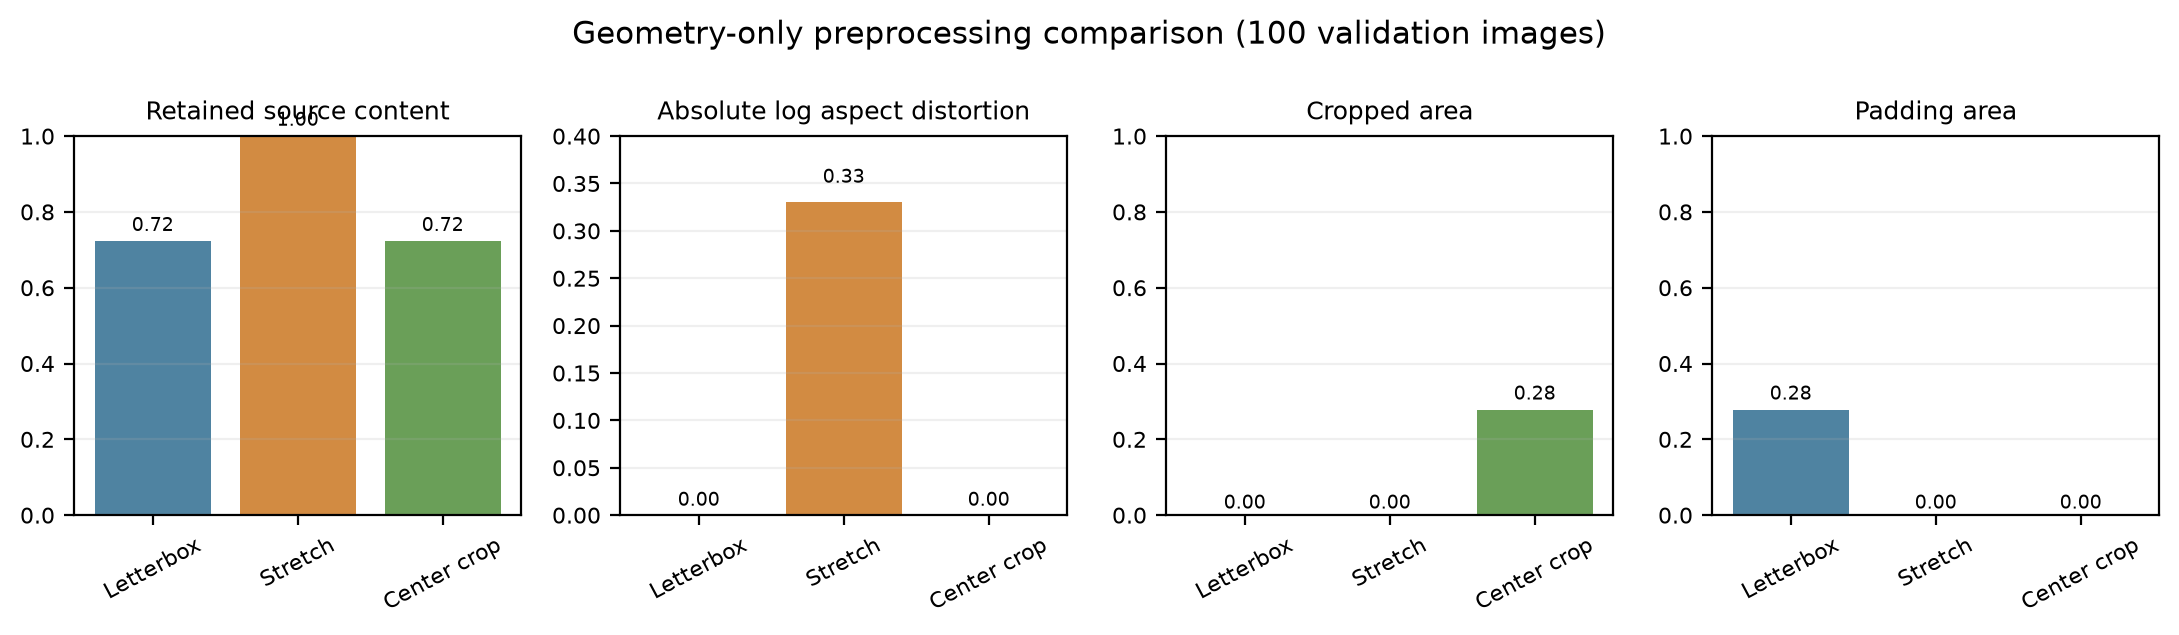
\includegraphics[width=0.94\textwidth]{preprocessing_geometry_summary.png}\caption{Geometry comparison on 100 validation images; no downstream model performance was measured.}\label{fig:preprocess}\end{figure}

\section{Quantitative Results}\label{ch:results}
The quality-control report records PASS for all applicable Phase 1 checks, with zero failed, warning, or not-run checks. It verifies 10,000/100/1,000 image records, corresponding 50,000/500/5,000 captions, complete image decoding, split disjointness, exact and perceptual hash checks, vector shapes/norms, mapping order, and FAISS readback. The summary is shown in \cref{tab:qc}. The report's PASS describes the checks implemented by the repository; it must not be read as full project or assignment completion.

\begin{table}[htbp]\centering\caption{Selected quality-control outcomes recorded by the project.}\label{tab:qc}
\begin{tabularx}{\textwidth}{lX}\toprule Check & Recorded result\\\midrule Processed-image decode & 11,100 decoded; 0 errors; 0 missing files\\Split overlap & 0 pairwise overlaps\\Exact duplicate check & 0 SHA-256 duplicate groups\\Perceptual duplicate audit & 11,100 hashed; 9 within-split candidates; 0 cross-split candidates at threshold 6\\Image embedding integrity & Train 10,000; validation 100; test 1,000; 512-D, finite, unit norm\\Caption embedding integrity & 50,000 train vectors; source order valid; held-out caption IDs: 0\\Index readback & Image 10,000 and caption 50,000; dimension 512; valid\\\bottomrule\end{tabularx}\end{table}

Image retrieval returned results for all 20 held-out queries, each with five neighbors, and no self-matches. The complete summary is in \cref{tab:retrieval}. Mean top-1 cosine similarity was 0.8260029644. The value measures similarity between CLIP image embeddings and training gallery items; without relevance judgments it does not quantify retrieval precision or caption quality. The caption index smoke test returned a nearest non-self caption with cosine 0.9504 for its first training caption query; this is a single construction check, not an aggregate evaluation.

\begin{table}[htbp]\centering\caption{Held-out image retrieval smoke test.}\label{tab:retrieval}
\begin{tabular}{lr}\toprule Measure & Value\\\midrule Queries & 20 (validation/test)\\Gallery & 10,000 train images\\Requested neighbors & 5\\Successful query results & 20/20\\Self matches & 0\\Mean top-1 cosine similarity & 0.8260\\Index readback & Valid\\\bottomrule\end{tabular}\end{table}

\section{Dataset Exploration}\label{ch:exploration}
\section{Object categories and scene complexity}
The train2017 annotation audit covers 80 object categories. Person instances account for 262,465 of 860,001 instances (30.52\%), followed by cars (43,867; 5.10\%) and chairs (38,491; 4.48\%). The distribution is long-tailed, as illustrated by the repository's top-50 frequency visualization (\cref{fig:cats}). Instance counts have mean 7.27 and median 4 in the complete train2017 annotation pool; counts range from zero to 93. Selected image complexity labels are based on source-pool quartiles of nonzero object count (Q1=2, Q3=10), not a learned scene-complexity model.

\begin{figure}[htbp]\centering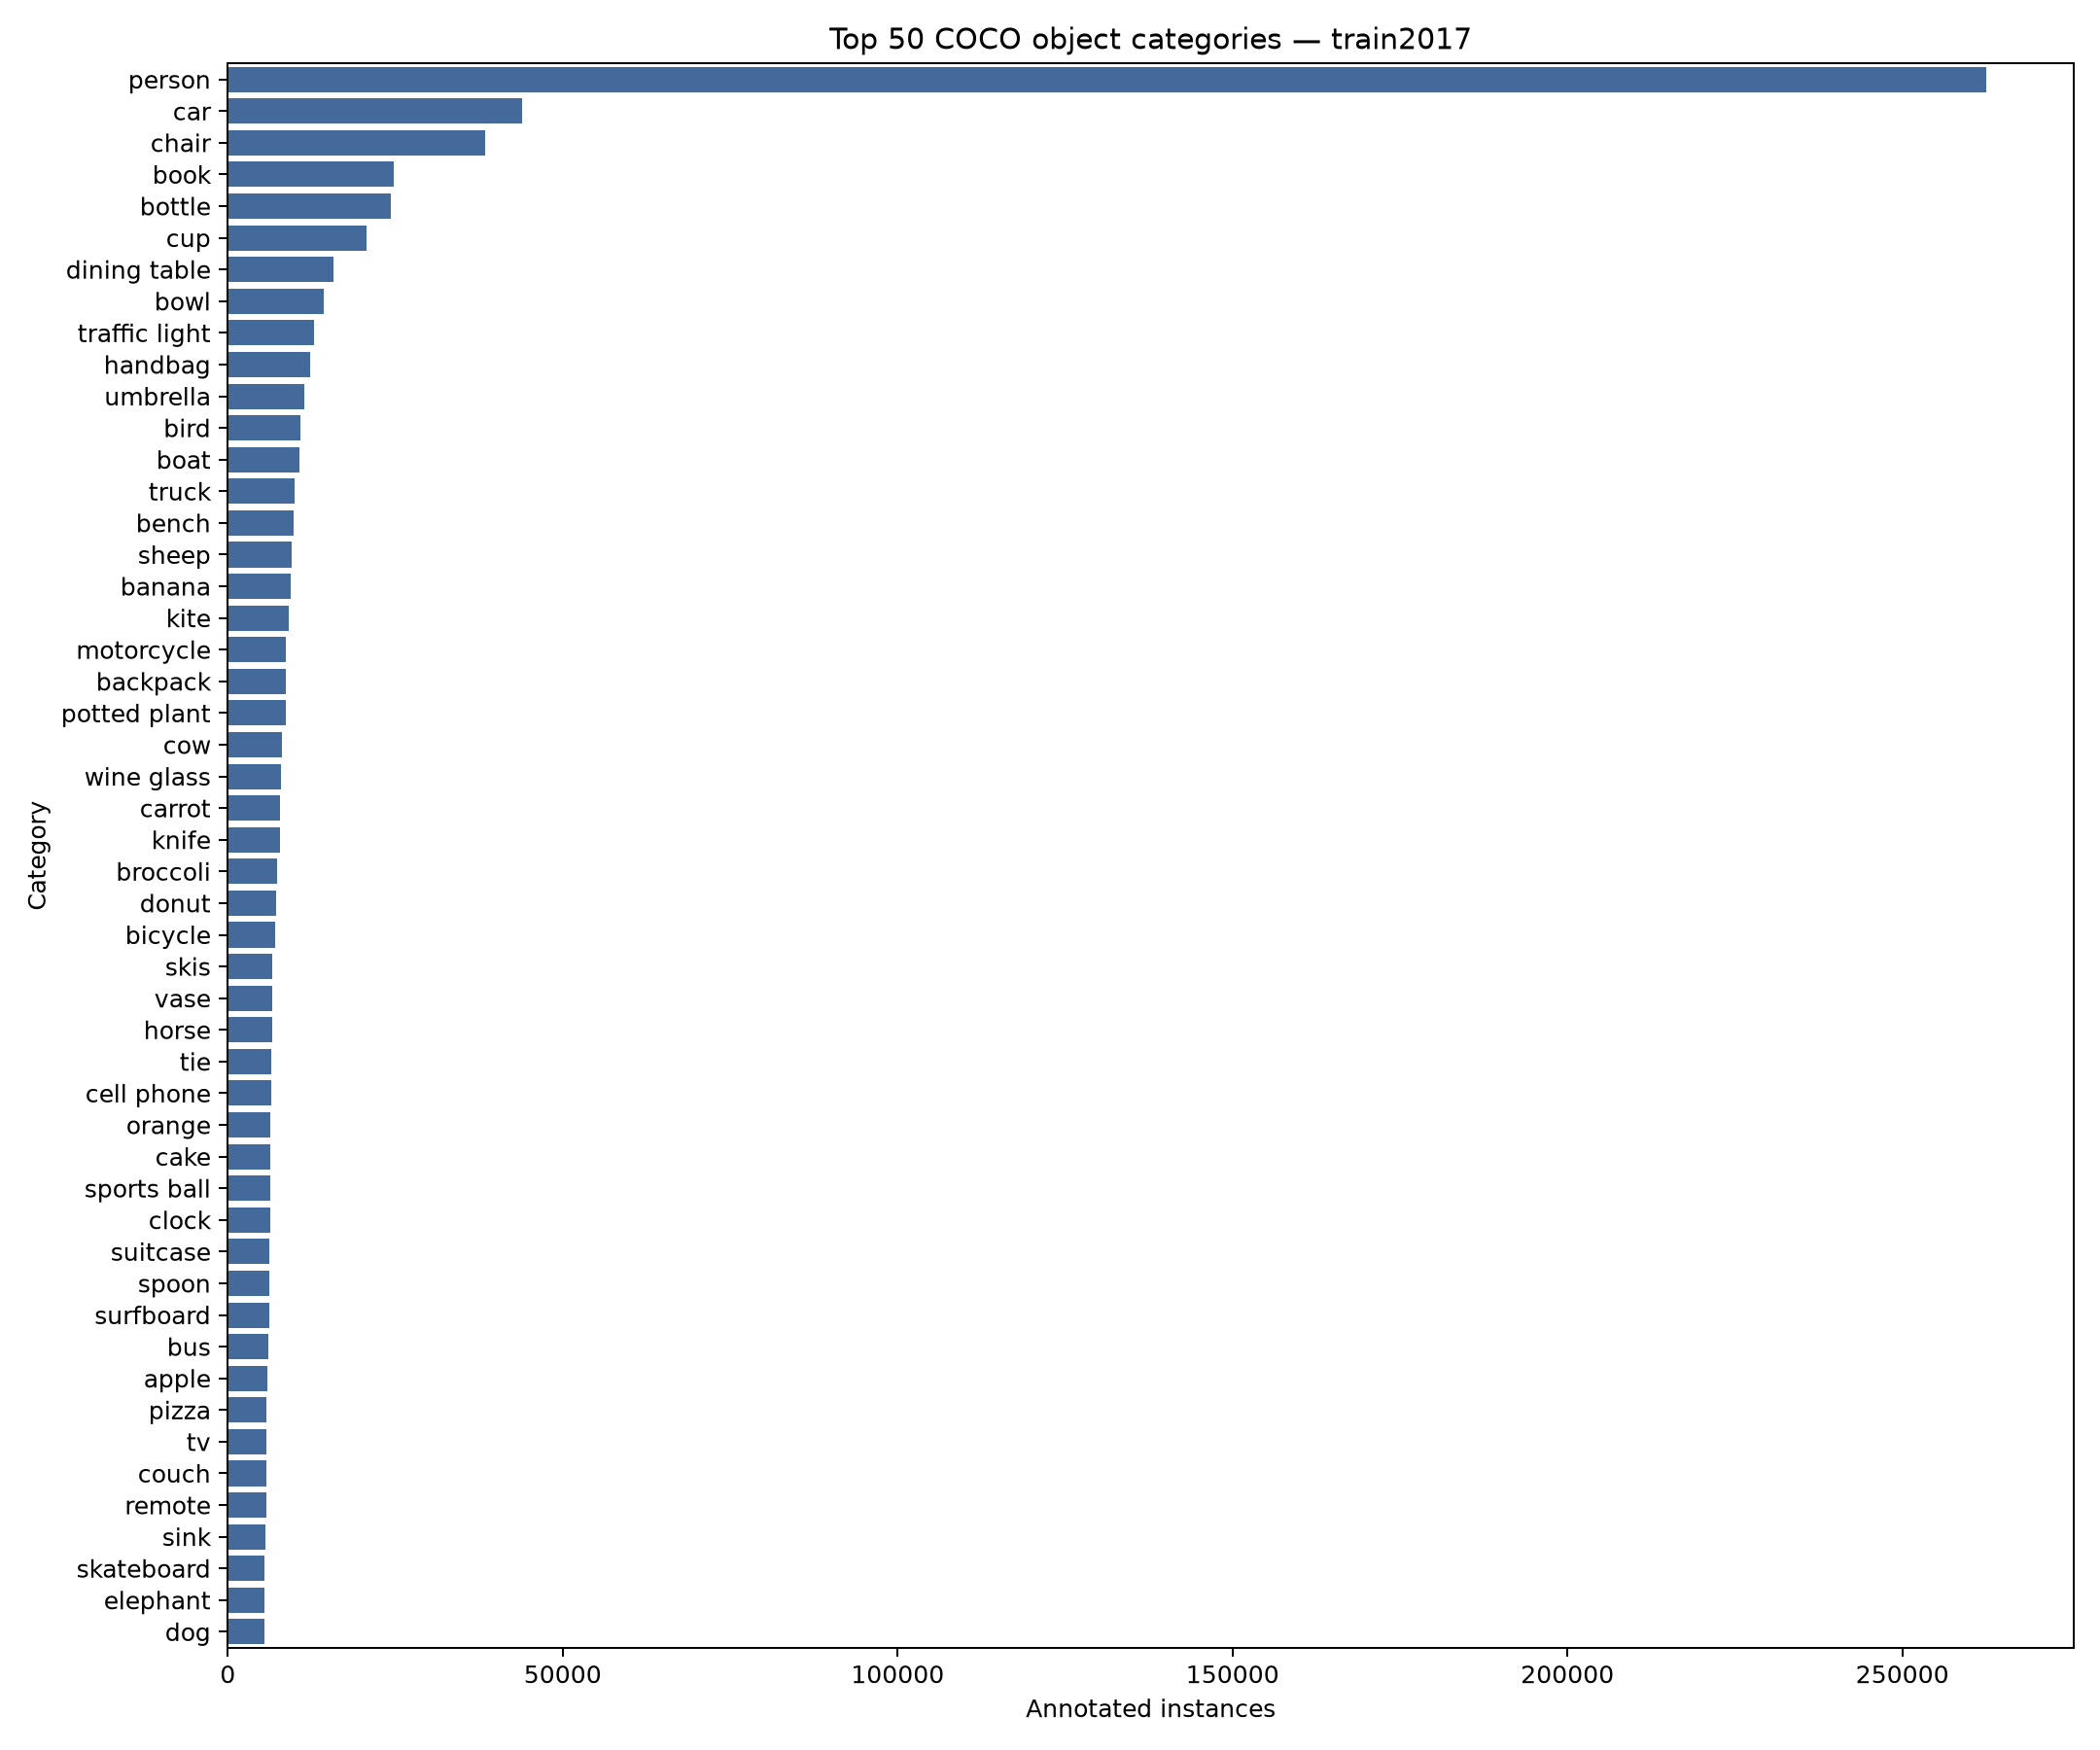
\includegraphics[width=0.88\textwidth]{top50_object_classes.png}\caption{Frequencies of the 50 most common COCO object categories in train2017 annotations. Annotation counts are not caption-generation results.}\label{fig:cats}\end{figure}

\section{Captions and vocabulary}
Every selected image has five references. A Unicode NFKC-normalized, case-folded tokenizer recognizes Unicode letters and numbers and retains internal apostrophes; it does not stem or lemmatize. Across all 55,500 references, the extended analysis reports 591,664 tokens and 9,793 unique tokens. A distinct spaCy POS stage covers 55,500 captions, records 642,147 model-tokenized tokens, and reports zero processing errors. The token totals differ because the analyses use different tokenization systems and definitions. They should not be conflated. Caption length, word frequency, and vocabulary-rank charts are available in the repository; example length and POS distributions are shown in \cref{fig:captions,fig:pos}.

\begin{figure}[htbp]\centering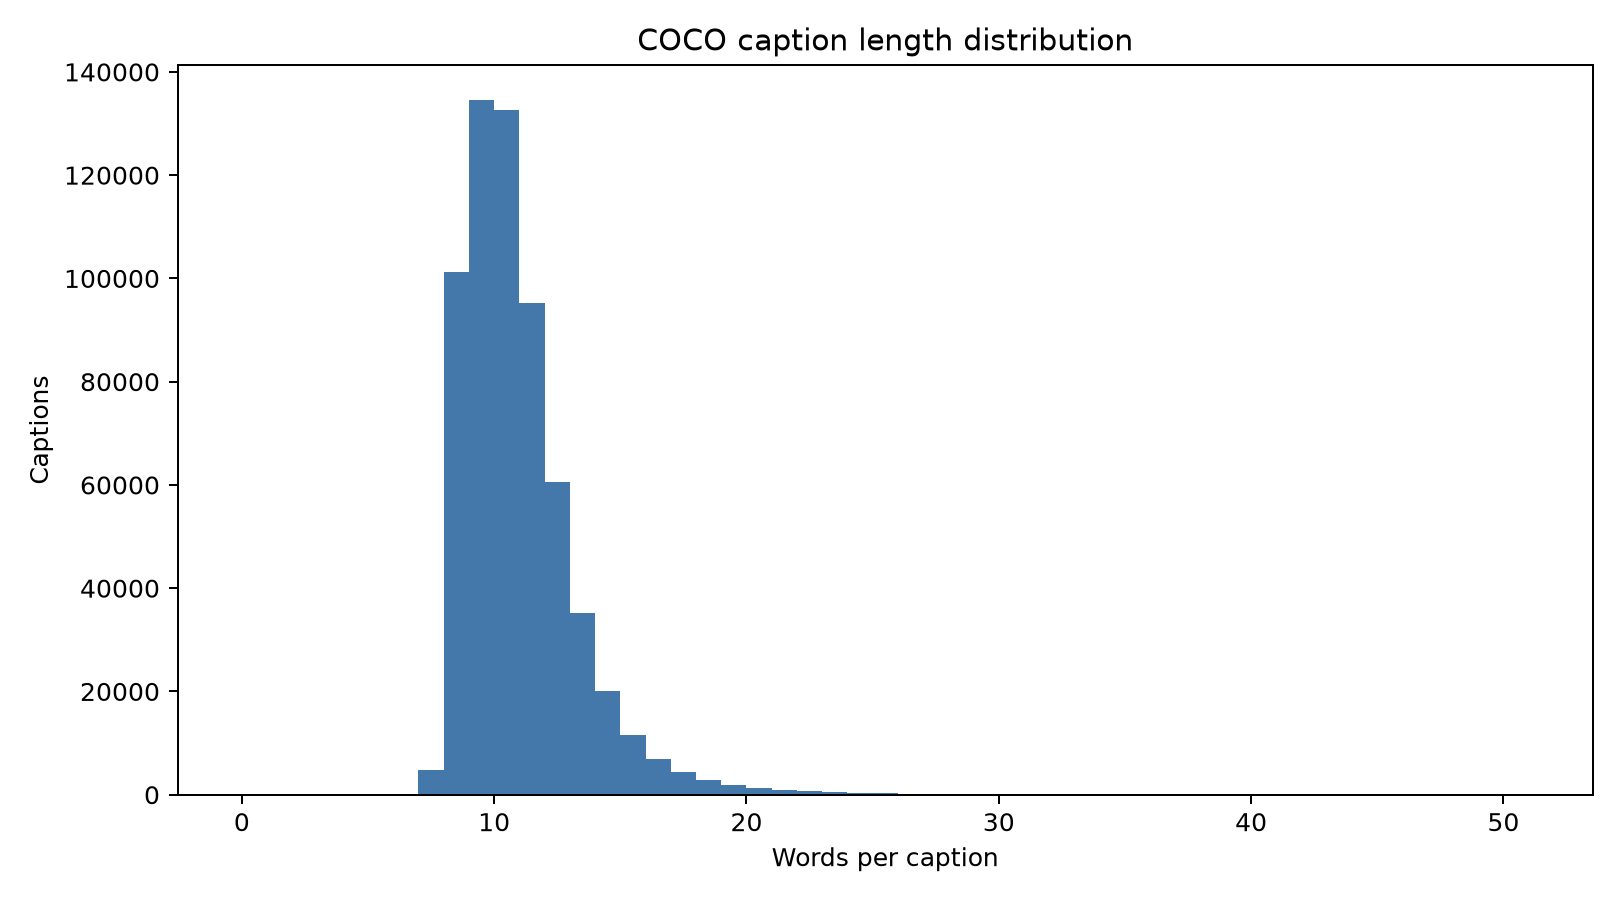
\includegraphics[width=0.8\textwidth]{caption_length_distribution.png}\caption{Caption-length distribution generated by the project caption analysis.}\label{fig:captions}\end{figure}
\begin{figure}[htbp]\centering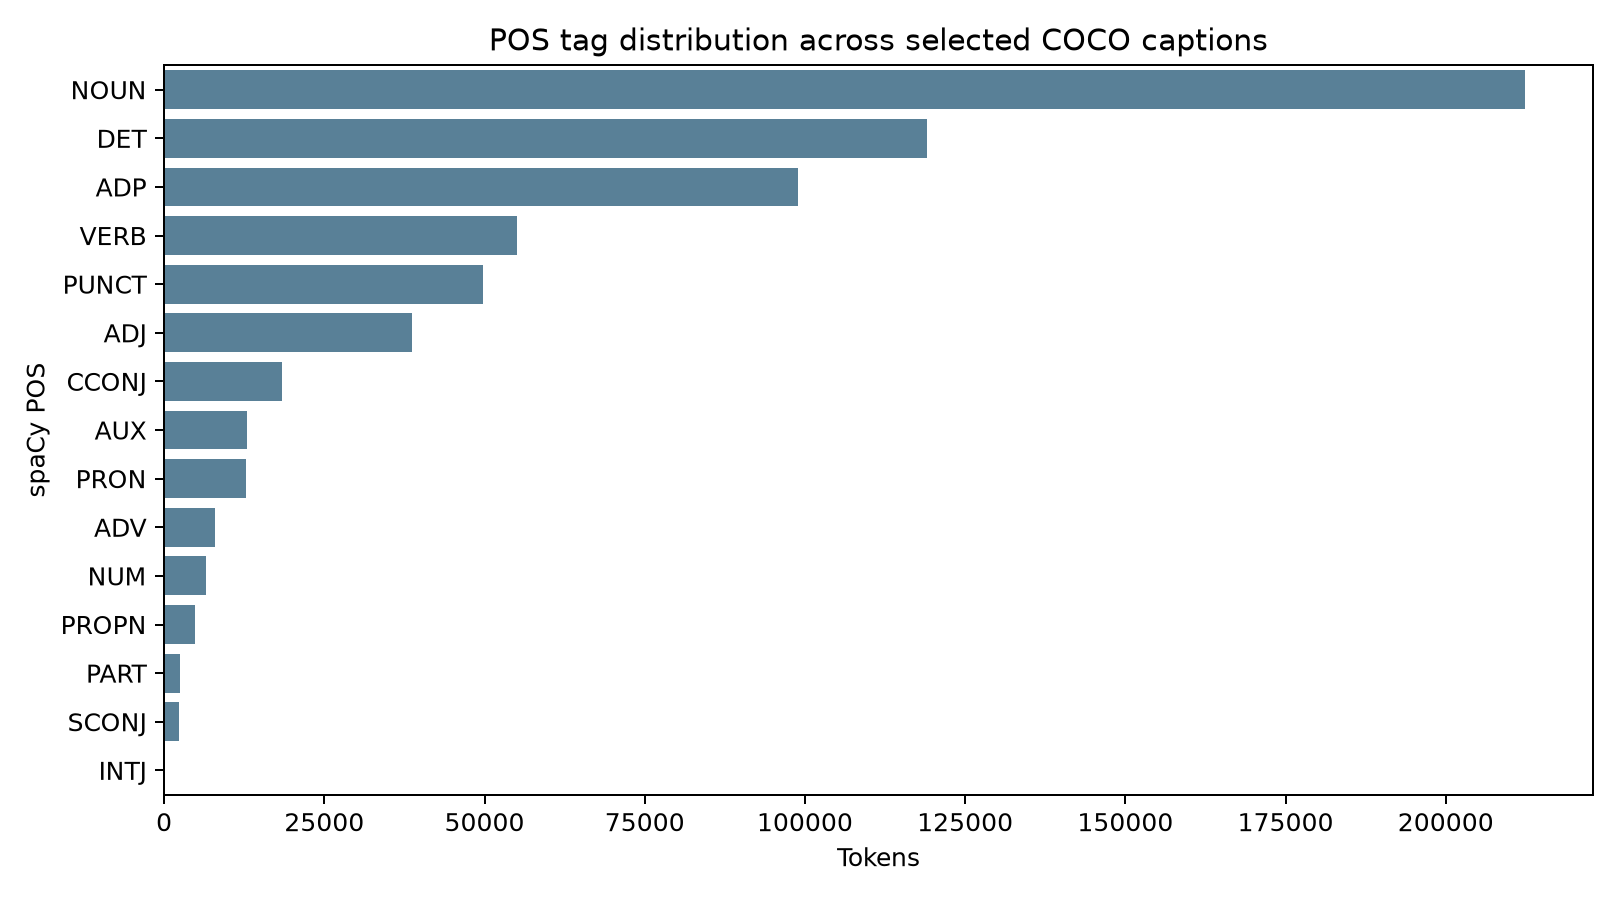
\includegraphics[width=0.8\textwidth]{caption_pos_distribution.png}\caption{spaCy part-of-speech token distribution across selected captions; tags are model predictions.}\label{fig:pos}\end{figure}

\section{Bounding-box geometry}
The project computes pairwise box relations from COCO instance boxes. It counts centroid ordering (left/right and above/below), containment, intersection-over-union overlap (IoU at least 0.10), and proximity by normalized center distance at most 0.10. Across 11,100 selected images the recorded pair counts include 680,482 left-of, 671,396 below, 676,706 right-of, 584,569 above, 47,381 overlapping, 151,587 near, 28,366 contains, and 30,359 inside. These are calculations over annotated object boxes, not COCO semantic relationship labels. They do not prove interaction, contact, support, or action. The relationship chart is presented as descriptive geometry only (\cref{fig:relations}).
\begin{figure}[htbp]\centering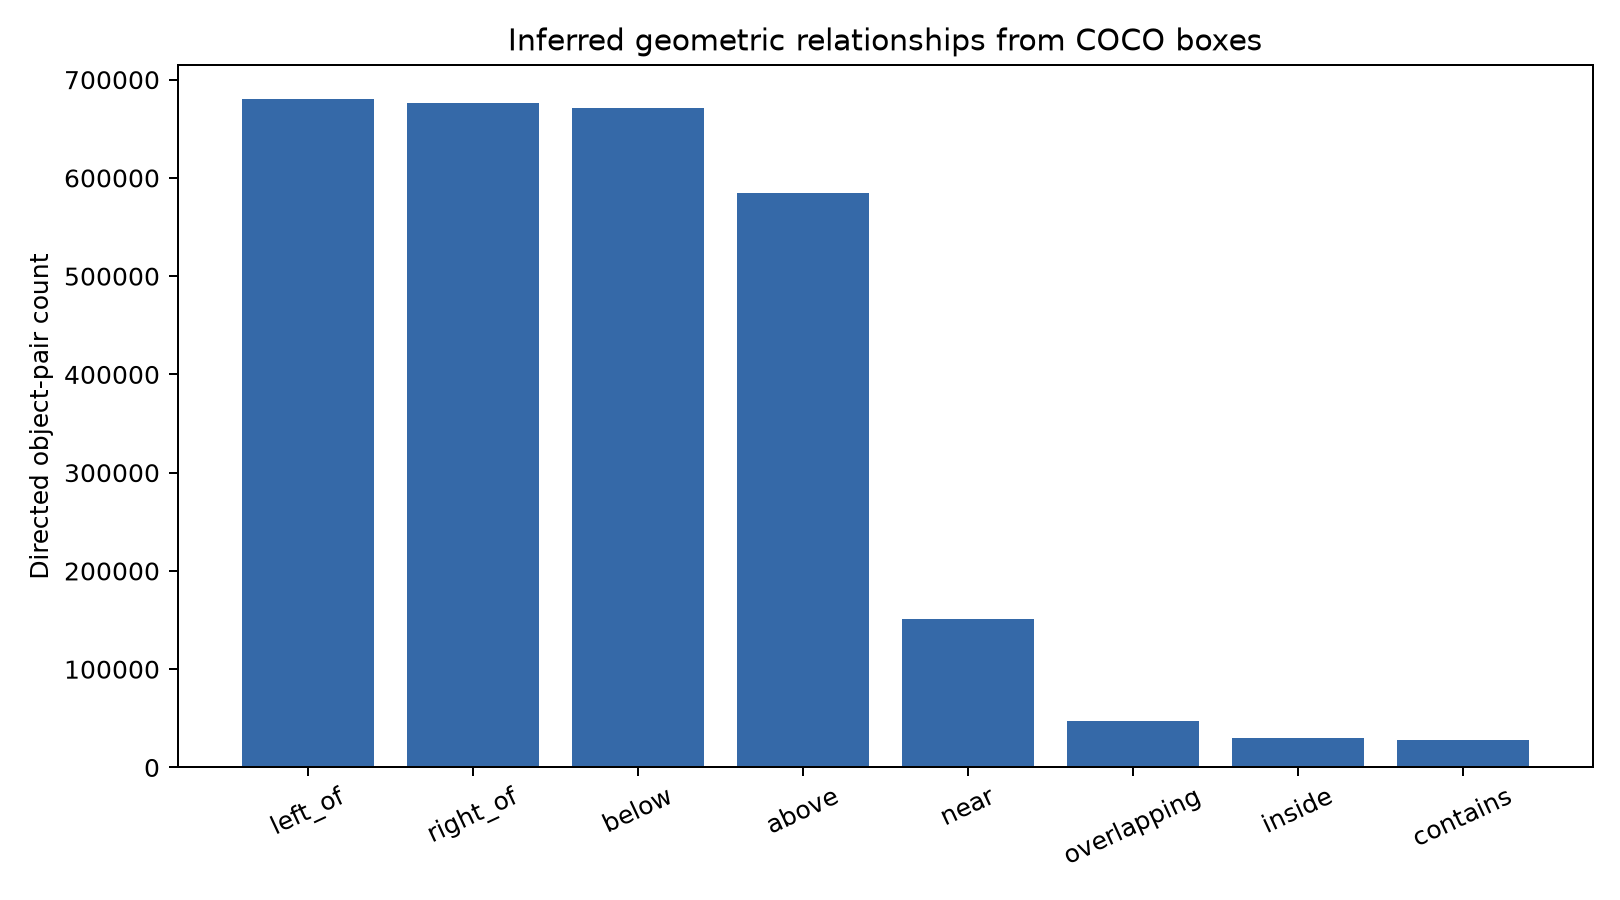
\includegraphics[width=0.88\textwidth]{geometric_relationship_frequencies.png}\caption{Counts of box-derived geometric relationships in selected images. Relation terms are operational geometric rules, not semantic ground truth.}\label{fig:relations}\end{figure}

\section{Pixel-level visual analysis}
The color analysis samples image pixels and maps hues to coarse color families; luminance and saturation summaries are image-level measures. Its dominant-color counts include red 4,430 and gray 3,948 images, with the remaining image counts spread among other color families. The method does not identify the color of a particular object. A global edge-density proxy uses image edges and is not object segmentation or shape recognition. Scene/context/day-night tags are zero-shot CLIP prompt predictions with confidence thresholds and abstention; their softmax scores are relative and uncalibrated. These sources are kept separate from COCO annotation labels. See \cref{fig:color,fig:scene}.
\begin{figure}[htbp]\centering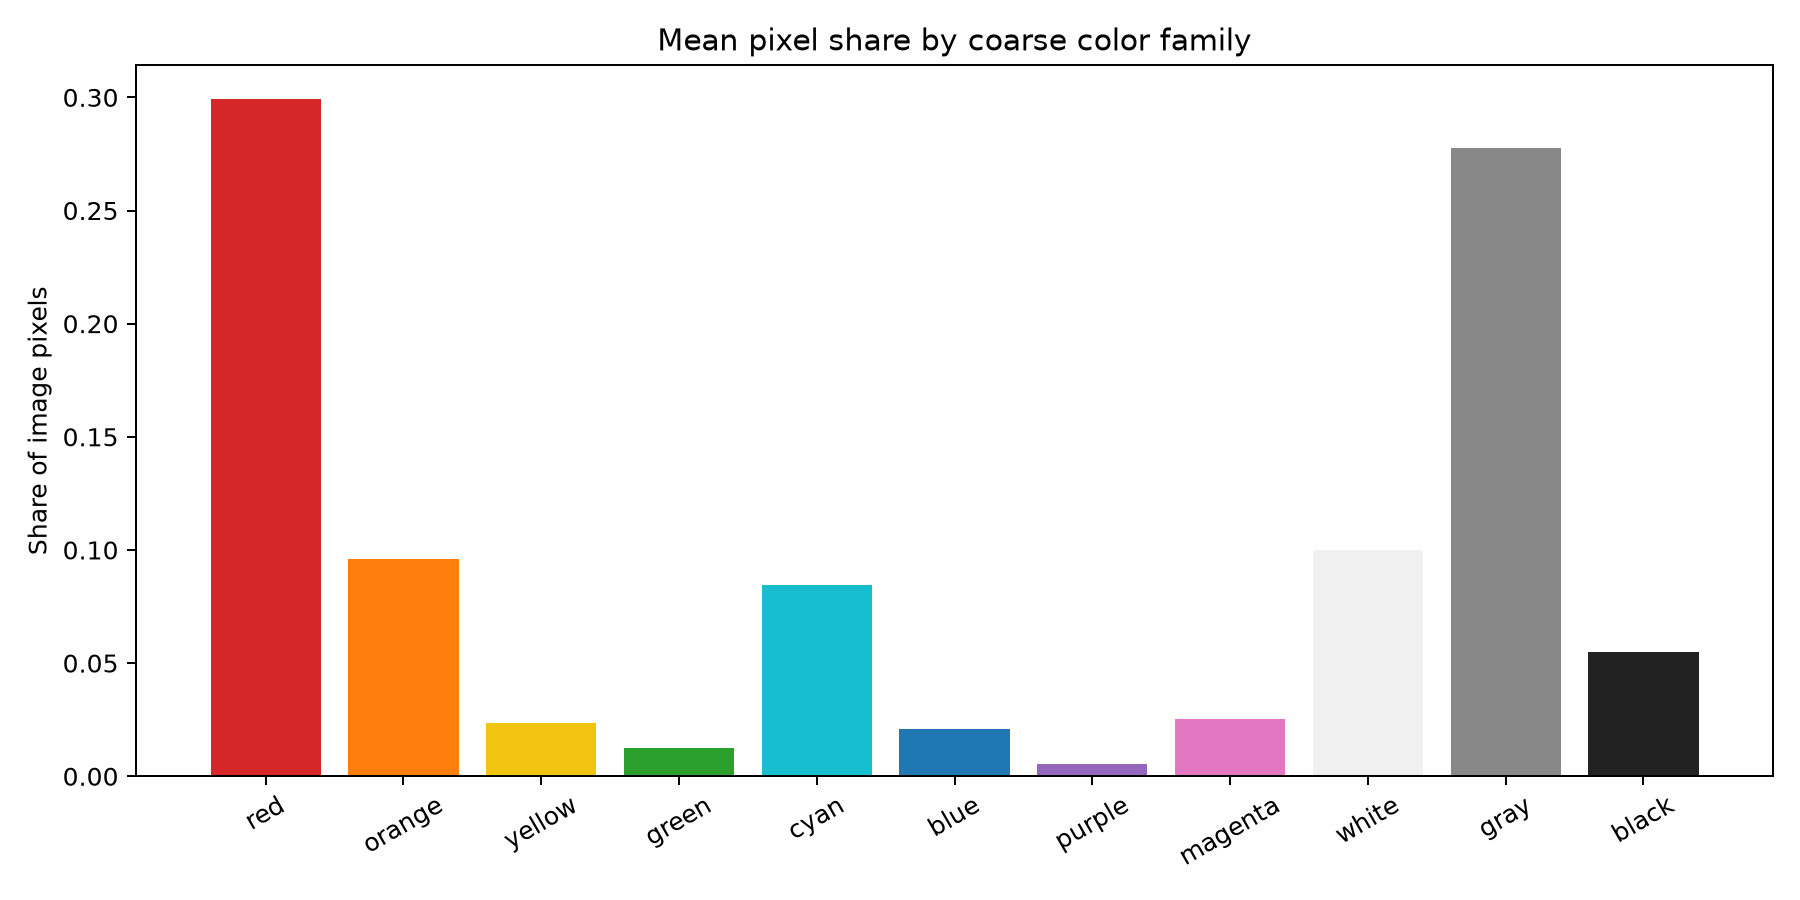
\includegraphics[width=0.78\textwidth]{color_family_distribution.png}\caption{Coarse dominant pixel-level color-family analysis over the selected images.}\label{fig:color}\end{figure}
\begin{figure}[htbp]\centering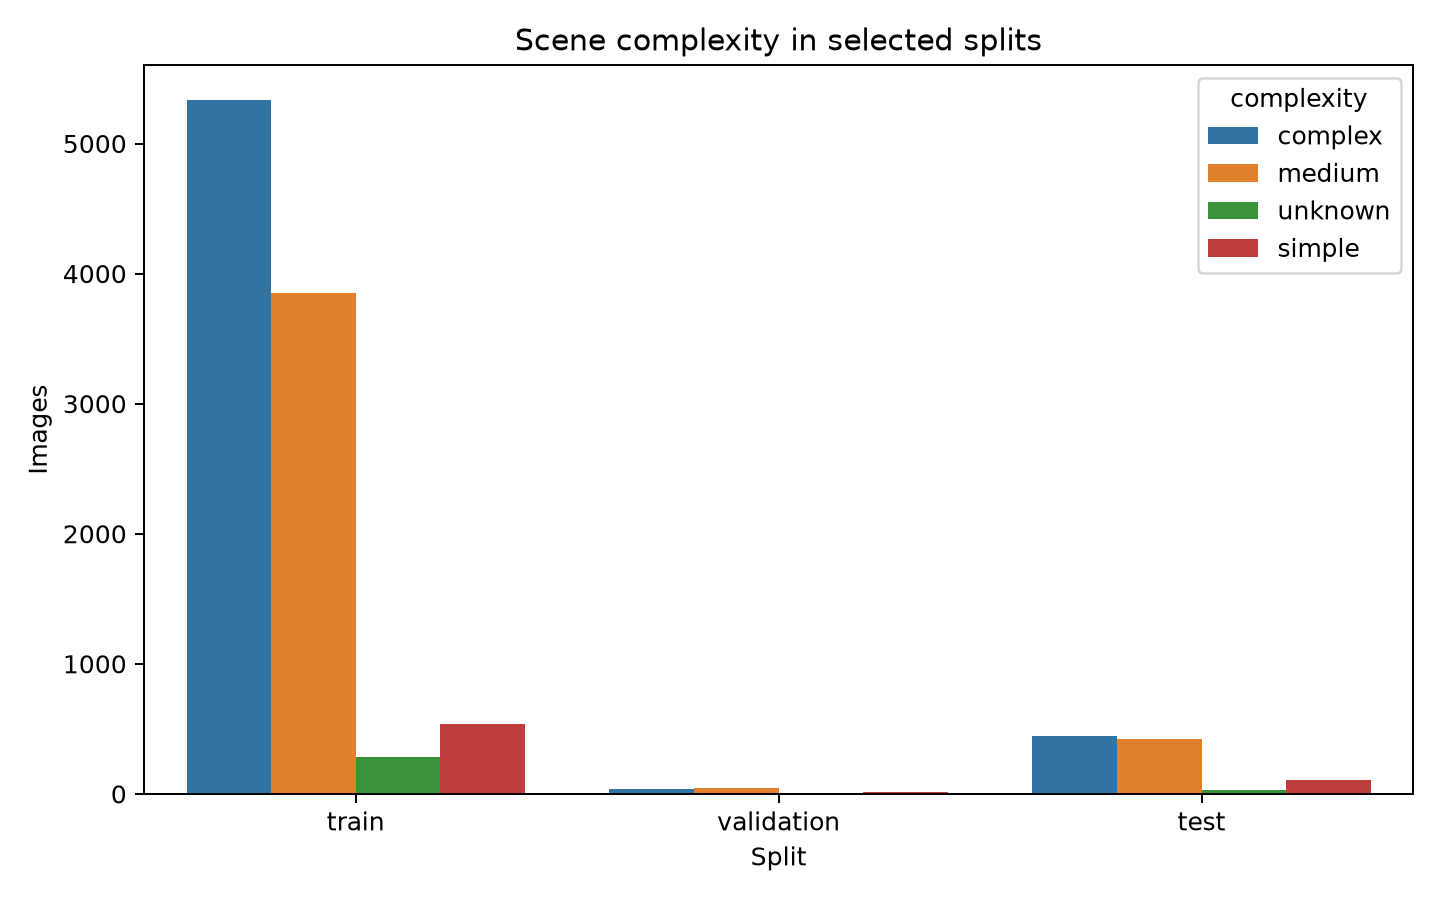
\includegraphics[width=0.78\textwidth]{selected_scene_complexity.png}\caption{Selected-image scene-complexity distribution based on annotation counts.}\label{fig:scene}\end{figure}

\chapter{Pending Generation Experiments}\label{ch:stats}
No inferential statistical tests have been performed for generated captions because no generation outputs exist. The project reports descriptive counts, means, distributions, and a retrieval similarity mean, but it has no paired metric vectors, human ratings, or method-level outcomes from which to calculate confidence intervals or significance tests. Accordingly, no p-values or claims of statistical significance are reported.

For the future paired comparison, each held-out image should be evaluated under every RAG condition with identical references. Report per-image metric differences and bootstrap confidence intervals. For metric distributions that support paired parametric inference, a paired test may be reported with effect size; otherwise use a paired nonparametric test such as Wilcoxon signed-rank, with correction for multiple comparisons. Human judgments should be analyzed with an appropriate repeated-measures or mixed-effects model. These are recommendations, not completed analyses.

\section{Ablation Analysis}\label{ch:ablation}
An ablation requires measured outputs under controlled variants. No caption generator or RAG method is implemented, so changing retrieval depth, removing retrieved evidence, altering the retrieved modality, or varying evidence formatting cannot yield valid caption-quality results in this repository. The geometry-only preprocessing comparison in \cref{tab:preprocess} is not a model ablation: it evaluates image geometry and does not measure a downstream task.

\begin{table}[htbp]\centering\caption{Planned ablation matrix; no metric values are available.}\label{tab:ablation}
\begin{tabularx}{\textwidth}{lXXX}\toprule Variant & Controlled change & Evaluation & Status\\\midrule No retrieval & Generator only & Caption metrics and grounding & \pending\\Image neighbors & Image-vector top-$k$ evidence & Same held-out set & \pending\\Caption neighbors & Text-vector top-$k$ evidence & Same held-out set & \pending\\Hybrid evidence & Image and caption evidence & Same held-out set & \pending\\Top-$k$ sensitivity & Vary $k$, fixed generator & Quality/faithfulness trade-off & \pending\\\bottomrule\end{tabularx}\end{table}

\section{Hallucination Analysis}\label{ch:hallucination}
Hallucination analysis should test whether a generated caption asserts objects, attributes, counts, actions, or relations unsupported by the image. The current project has no generated captions and no hallucination annotations, so a hallucination rate cannot be calculated. COCO category labels and boxes may support object-presence checks but do not provide exhaustive scene truth: an unannotated object is not necessarily absent, and a box does not establish an action or relation. CLIP similarity alone is not a reliable factuality validator.

A future protocol should define claim categories before evaluation, annotate a stratified sample with independent raters, assess agreement, and compare generated claims against image evidence. Automated object consistency can be reported separately from human judgments and should include known annotation-coverage limitations. No fabricated hallucination scores are included.

\section{Qualitative Analysis}\label{ch:qualitative}
The repository includes qualitative retrieval records and visual audit materials, but it does not produce captions for qualitative comparison. Retrieval neighbors can be inspected to identify plausible visual analogies and failure cases, yet similarity scores do not prove that the retrieved caption is appropriate for the query. No fabricated image-caption examples are presented as experimental outputs.

Future qualitative review should sample successes and failures across scene complexity and object-frequency strata. It should show the query image, retrieved images/captions, generated output, reference captions, and a concise judgment of evidence support. The existing analyses indicate useful dimensions for this review: object count, category mix, color family, scene predictions, and caption lexical patterns. Zero-shot scene tags and inferred geometric relations should be visibly marked as model-derived or computed metadata.

\chapter{Discussion and Conclusions}\label{ch:discussion}
The main demonstrated contribution is a reproducible Phase 1 substrate: fixed image splits and caption references, explicit provenance-oriented metadata, normalized visual and text embeddings, separate training-only indexes, and integrity checks. The retrieval smoke test shows that the stored image vectors can be searched and that the tested held-out queries do not retrieve themselves. This confirms pipeline operation under the recorded configuration.

Several boundaries matter for interpretation. The 0.8260 mean top-1 cosine is a similarity statistic without judged relevance labels. The successful QC status covers implemented checks, not the complete academic project. CLIP scene predictions are not calibrated; box relations are geometric; color and edge metrics are coarse image-level proxies. The selected 100-image validation set is small for broad statistical conclusions, and the 20-query smoke test is intended as a functional check rather than a benchmark. Full-scale retrieval relevance and generation quality remain unmeasured.

The two memory types create an opportunity for a controlled study. Image memory could retrieve visual neighbors; caption memory could retrieve language examples. A proper experiment must prevent the query's own references from entering its evidence, preserve train-only knowledge, keep generator settings fixed, and inspect whether retrieved examples help or propagate errors. The current separation of training and held-out data is a sound prerequisite, but prompt and generation leakage controls still need implementation.

\section{Limitations}\label{ch:limits}
The most important limitation is scope: Phase 2 is absent. There is no caption decoder, no RAG prompt assembly, no comparative method, no generation evaluation, no significance test, no ablation, and no hallucination study. There is also no original assignment PDF in the audited project locations, so the report cannot verify exact professor wording or the designated technique. The 100-versus-1,000 test-size conflict remains unresolved; the repository uses 1,000.

Reproducibility is partial. The seed, model identifier/revision, key tensor properties, and many artifact mappings are recorded, but a unified environment snapshot is missing. Historical counts of EXIF corrections and grayscale/RGBA conversions were not retained. The metadata audit flags raw-caption mapping integrity as partial even though five-per-image cardinality and current record counts pass. The preprocessing comparison was created for the audit and evaluates geometry only. These gaps should be addressed before the final comparative study.

Dataset limitations include the restricted 11,100-image sample and COCO's incomplete annotation coverage. Text token counts depend on tokenization. POS and zero-shot scene outputs may be wrong. Perceptual hash candidates indicate visual similarity rather than confirmed identity. These constraints limit claims to the observed artifacts and prevent strong generalization or causal statements.

\section{Conclusion and Next Steps}\label{ch:conclusion}
The repository contains a complete and quality-controlled Phase 1 preparation pipeline for a proposed RAG image-captioning study. It selects 10,000 training, 100 validation, and 1,000 test images, preserves five captions per image, prepares letterboxed RGB inputs, analyzes annotations and visual/text properties, extracts 512-dimensional normalized CLIP vectors, builds train-only image and caption indexes, and validates held-out image retrieval on 20 queries. Integrity checks report no split overlap, no exact duplicates, and no cross-split perceptual candidates at the configured threshold.

These findings establish data and retrieval readiness, not improved caption generation. The central comparative research question remains unanswered because generation experiments are pending. The next phase should obtain instructor clarification on test size and assigned technique; freeze an explicit generator and baseline; implement controlled image-, caption-, and hybrid-retrieval conditions; exclude query-associated references; evaluate with multiple complementary metrics and human grounding judgments; analyze paired outcomes and ablations; and publish complete configurations and outputs. Until then, all caption-quality claims must remain open.

\appendix

\appendix
% Compatibility entry point; active appendix source: appendix_artifacts_new.tex.
\section{Reproducibility Summary}
\label{app:reproducibility}
\begin{table}[H]
\centering
\small
\caption{Compact configuration and reproducibility record.}
\label{tab:configuration}
\rowcolors{2}{ProjectGrey}{white}
\begin{tabularx}{\textwidth}{@{}>{\raggedright\arraybackslash}p{0.30\textwidth}X@{}}
\toprule
\textbf{Setting} & \textbf{Recorded value}\\
\midrule
Selection seed & 20261106\\
Image input & 224 by 224 pixels; RGB; black letterbox padding\\
Image format & JPEG\\
Image and text model & \code{openai/clip-vit-base-patch32}\\
Recorded model revision & \url{3d74acf9a28c67741b2f4f2ea7635f0aaf6f0268}\\
Embedding dimension and type & 512; float32\\
Normalization & L2; unit-length vectors\\
Batch size & 64\\
Text maximum sequence length & 77 tokens\\
Image index & FAISS \code{IndexFlatIP}; train gallery\\
Caption index & FAISS \code{IndexFlatIP}; train captions only\\
Retrieval settings & top-\(k=5\); 20 held-out query smoke test\\
POS model & spaCy \code{en\_core\_web\_sm}\\
Run environment & CPU; PyTorch 2.15.0+cpu; Transformers 5.22.1\\
Execution time & 1,121.3 seconds for training-caption embeddings\\
Split manifests & Frozen JSON/CSV files under \code{data/selected/}\\
Report build & Tectonic 0.17.0; \code{tectonic main.tex}\\
\bottomrule
\end{tabularx}
\end{table}

The authoritative parameters are in \code{configs/config.json}; frozen split IDs are in \code{data/selected/}. Embeddings, mappings, and FAISS indexes are saved under \code{embeddings/} and \code{vector\_database/}. The saved caption-vector run records CPU execution, PyTorch 2.15.0+cpu, Transformers 5.22.1, and 1,121.3 seconds. A complete unified environment snapshot was not available, so these versions should not be treated as a full environment lock.

The report was built with Tectonic 0.17.0. From this directory, compile using \code{tectonic main.tex}; the Python pipeline itself is not rerun to build the report.

\endinput
\chapter{Reproducibility and Artifact Map}
\begin{itemize}[leftmargin=1.7em]
\item Configuration: \nolinkurl{configs/config.json}; source stages: \nolinkurl{src/pipeline.py}, \nolinkurl{src/embeddings.py}, \nolinkurl{src/text_embeddings.py}, \nolinkurl{src/retrieval.py}, \nolinkurl{src/quality_control.py}, \nolinkurl{src/extended_analysis.py}, \nolinkurl{src/visual_analysis.py}, and \nolinkurl{src/perceptual_hash.py}.
\item Frozen manifests: \nolinkurl{data/selected/}; images: \nolinkurl{data/processed/}; metadata and captions: \nolinkurl{data/metadata/} and \nolinkurl{data/captions/}.
\item Embeddings and indexes: \nolinkurl{embeddings/} and \nolinkurl{vector_database/}.
\item Quality evidence: \nolinkurl{reports/final_quality_control.json}, \nolinkurl{reports/phase1_final_compliance.json}, and \nolinkurl{reports/PHASE1_FINAL_COMPLIANCE_REPORT.md}.
\end{itemize}

\chapter{Pending Results Template}
The following quantities must be filled only after generation experiments are run. No placeholder below represents a measured result.
\begin{table}[htbp]\centering\caption{Generation evaluation results: pending.}\label{tab:pending}
\begin{tabular}{lrrrrrr}\toprule Method & BLEU & METEOR & ROUGE-L & CIDEr & SPICE & BERTScore\\\midrule No retrieval & -- & -- & -- & -- & -- & --\\Image retrieval & -- & -- & -- & -- & -- & --\\Caption retrieval & -- & -- & -- & -- & -- & --\\Hybrid retrieval & -- & -- & -- & -- & -- & --\\\bottomrule\end{tabular}\end{table}

\bibliographystyle{plainnat}\bibliography{references}
\end{document}
